\section{Semantics in a Dynamic Network}
\label{sec:dynamic}

In practice, the state of the network is constantly changing during
query execution. In contrast to transactional databases, changes to
network state are not isolated from queries
while they are running.  Instead, as in network protocols, queries
are expected to perform dynamic recomputations to reflect the most current state of the
network. To better understand the semantics in a dynamic network, we
consider the following two degrees of dynamism:   

%\begin{mylist}
\vspace{1pt}

\noindent {\bf Continuous Update Model: }In this model, we assume that
updates occur very frequently -- at a period that is shorter than the
expected time for a typical query to reach a fixpoint. Hence, the query
results never fully reflect the state of the network.
 
\vspace{1pt}
\noindent {\bf Bursty Update Model: }In this idealized (but still fairly realistic model), updates are allowed
  to happen during query processing.  However, we make the assumption
  that after a burst of updates, the network eventually {\em quiesces}
  (does not change) for a time long enough to allow all the
  queries in the system to reach a fixpoint. 
%\vspace{1pt}
%\end{mylist}

In our analysis, we focus on the bursty model, since it is amenable to
analysis; our results on that model provide some intuition as to the
behavior in the continuous update model.  Our goal in the bursty model
is to achieve a variant of the typical distributed systems notion of {\em eventual
  consistency}, customized to the particulars of \Dlog: we wish to
ensure that the eventual state of the quiescent system corresponds to
what would be achieved by rerunning the queries from scratch
in that state. We briefly sketch the ideas here, and follow up with
details in the remainder of the section.  

To ensure well-defined semantics, we use techniques from materialized view
maintenance~\cite{viewIncremental}, and consider three types of changes:

%\begin{mylist} 
\vspace{1pt}

\noindent {\bf Insertion: } The insertion of a new tuple at any stage of
  processing can be naturally handled by (pipelined) semi-\naive evaluation. 

\vspace{1pt}

\noindent {\bf Deletion: }The deletion of a base tuple leads to the
  deletion of any tuples that were derived from that
  base tuple.  Deletions are carried out incrementally via (pipelined)
  semi-\naive
  evaluation by incrementally deriving all tuples that are to be
  deleted. 

\vspace{1pt}

\noindent {\bf Update: }An update is treated as a deletion followed by an
  insertion. An update to a base tuple may itself result in derivation
  of more updates that are propagated via (pipelined)
  semi-\naive evaluation. 
%We allow updates to base tables where a new tuple replaces an existing
%  tuple with the same primary key. 
\vspace{1pt}
%\end{mylist}

%If the declared primary key does not include the full set of attributes,
%it is necessary to remember all possible tuples for each primary
%key, to handle updates. For instance, invalidation of the tuple for
%the current result might reveal another tuple with the same primary
%key value. Another important case arises in the distributed setting:
%updates arriving along different paths may be reordered, which can lead
%to temporarily having derivations of multiple tuples with identical
%primary keys.

%In addition,
The use of pipelined semi-\naive evaluation in the discussion can be replaced with
buffered semi-\naive without changing our analysis.
Since some tuples may have multiple derivations, we use the
{\em count algorithm}~\cite{viewIncremental} for keeping track of the
number of derivations for each tuple, and only delete a tuple when the
count is 0.

In dealing with queries with aggregates, we apply techniques for incremental computation of
aggregates~\cite{rossAggregate} in the presence of updates. The arrival of new
tuples may invalidate existing aggregates, and incremental
recomputations are cheaper than computing the entire aggregate from
scratch. For example, the re-evaluation cost for min and max aggregates are shown
to be $O(log$ $n)$ time and $O(n)$ space for the min and max
aggregates~\cite{rossAggregate}. 
%, and $O(1)$ in time and space for sum and count,
%where n is the size of the input. 


\subsection{Centralized Semantics}

We first provide an intuitive example for the centralized
case. Figure~\ref{Derivation Tree} shows a {\em derivation tree} for $path({\bf
  e},e,a,[e,a,b,e],7)$ based on the shortest-path
  query. The leaves in
  the tree are the $link$ base tuples. The root and
  the intermediate nodes are tuples recursively derived from the
  children inputs by applying either rules SP1 and SP2. When
updates occur to the base tuples, changes are propagated up the tree to
the root. For example, when the cost of $\#link({\bf a},b,5)$ is updated from $5$ to $1$,
$path({\bf a},b,e,[a,b,e],2)$ and $path({\bf e},a,[e,a,b,e],3)$ are re-derived
and replace the previous tuples. Similarly, the deletion of $link({\bf
  b},e,1)$ leads to the deletion of $path({\bf b},e,e,[b,e],1)$,
\\$path({\bf a},b,e,[a,b,e],2)$, and then $path({\bf e},a,e,[e,a,b,e],3)$.

Let $FP_{p}$ be the set of tuples derived using PSN under the bursty model,
and $FFP_{p}$ be the set of tuples that would be computed by PSN if
starting from the quiesced state. In Appendix~\ref{appendix:burstyCentral}, we
prove the following theorem:

\vspace{1pt}
\noindent{\bf Theorem~\ref{theorem:burst}: } {\em $FP_{p} = FFP_{p}$ in
  a centralized setting.}
\vspace{1pt}

The proof requires that all changes (inserts, deletes, updates) are applied in the same order
in which they arrive. This is guaranteed by the FIFO queue of PSN and
the use of timestamps.

\begin{figure}[ht]
\centering
\epsfig{file=images/dtree.eps, width=3.5in}
\caption{\label{Derivation Tree}\emph{\small Derivation tree for derived
    path tuple from a to e. The left diagram shows updating the tree due
    to a change in base tuple $\#link({\bf a},b,5)$, and the right diagram shows
    the deletion of $\#link({\bf b},e,1)$.}}
\end{figure}                                              

%\footnote{In the case of BSN, on top of using
%  timestamps, we have to ensure that there are no two updates involving
%  tuples of the same primary key within a set that is being processed}.

%Let $t(0)$ denotes the initial value of tuple $t$, and $t(j)$ denotes the $j^{th}$ updated value of $t$.
%Let $tree(t)$ be the derivation tree (defined in Appendix~\ref{appendix:bursty}) for t with n leaf nodes,
%$l_{1}(0),l_{2}(0),...,l_{n}(0)$. Suppose each leaf has $u_{k}$ updates
%each. At the end of the updates, the $k^{th}$ leaf is
%$l_{k}(u_{k})$. Let $finalTree(t)$ be another derivation tree for t with n leaf nodes, where the $k^{th}$ leaf is
%initialize to $l'_{k}(0)=l_{k}(u_{k})$ for each of the leaf nodes. 
%The theorem means that for a given derivation tree whose leaf nodes are
%subjected to changes, if updates along any ``edge'' in the tree is
%applied in order, the eventual result at the root of the tree is based
%on the final state of the leaves. 

\subsection{Distributed Semantics}

In order for incremental evaluation to work in a distributed
  environment, it is essential that along any link in the network, there
  is a FIFO ordering of messages. That is, along any link literal \link(s,d), facts
  derived at node s should arrive at node d in the same order in which they
  are derived (and vice versa). This guarantees that updates can be
  applied in order. Using the same definition of $FP_{p}$ and $FFP_{p}$ as before, assuming the link FIFO ordering, in Appendix~\ref{appendix:burstyDistributed}, we prove the following
theorem:

\noindent{\bf Theorem ~\ref{theorem:netburst}: } {\em $FP_{p} = FFP_{p}$
in a distributed setting with FIFO links. }

%In fact, if we allow relax the link-restricted requirement of \Dlog and
%allow all nodes to communicate directly with each other, having the FIFO link ordering is not sufficient to
%guarantee eventual consistency.
The drawback of enforcing network link FIFO is that it increases the
  complexity and lowers the performance of the underlying network. The
  alternative adopted by network protocols is to maintain all tuples as
  {\em soft state}. In the soft state storage model, all data (base
  and derived tuples) has an explicit ``time to live'' (TTL), and
  facts (in our case base tuples) must be explicitly reinserted with
  their latest values and a new TTL or they are deleted. Reinsertion
  of base tuples
  leads to recomputation of query results, which in a quiescent
  network, leads to eventual consistency through the reinsertion of
  the facts from the quiescent state. 
  The drawbacks of soft state are well known:  recomputation can be expensive, and
  if done only periodically, the time to react to failures is a half-period on
  average.  However, soft state is often favored in networking
  implementations because in a very simple manner it provides eventually correct semantics in
  the face of reordered messages, node disconnection, and
  other unpredictable occurrences.\\


%\item {\bf Unique Derivation.} Each tuple sent as a message should have
%  a unique derivation. \Eg in the shortest-path query, all generated
%  $path$ tuples have a unique derivation (due the the path being
%  stored). This guarantees that we can differentiate tuples that are
%  derived along different paths in the network.


%\item {\bf Sender Address.} Each tuple that is
%  sent over the network during query execution must include the
%  immediate sender's address field at each hop.  \Eg in the
%  shortest-path query, all generated $path$ tuples include {\em nextHop}
%  field. The purpose of including this field is to allow
%  identical tuples that are derived along different paths to be
%  differentiated. This constraint can be checked by making sure all rule
%  heads include both address fields of the \link predicate.

%This requirement serves
%  two purposes. First, this allows tuples sent along different paths to
%  be differentiated. Second, this allows the deletion of facts
%  belongling to a neighbor whose link has been disconnected.
%  derived tuples that was previously sent by the neighbor. 
%This can be enforced on
%  all localized link-restricted rule heads by assigning the \link.@S
%  address field as one of the output attributes in the head.
%This is enforced on all
%  link-stricted rules that must include the locational specifier of the
%  body predicates.

%\end{mylist}
% the query, since derived tuples may need
%to be sent across the network, the FIFO ordering imposed by a local
%queue no longer holds, due to message reordering imposed by network
%delays and also losses. For example, it is conceivable that node {\em e}
% receives the older $path({\bf e},a,b,[e,a,c,d],3)$ before the newer path
% $path({\bf e},a,b,[e,a,c,d],2)$ due to reordering of
%  the $path$ tuples sent from node {\em a}, and hence computes the final
%  $shortestPath(e,b,[e,a,c,d],3)$ that does not reflect the latest state
%  of the network.



%\begin{figure}[ht]
%\centering
%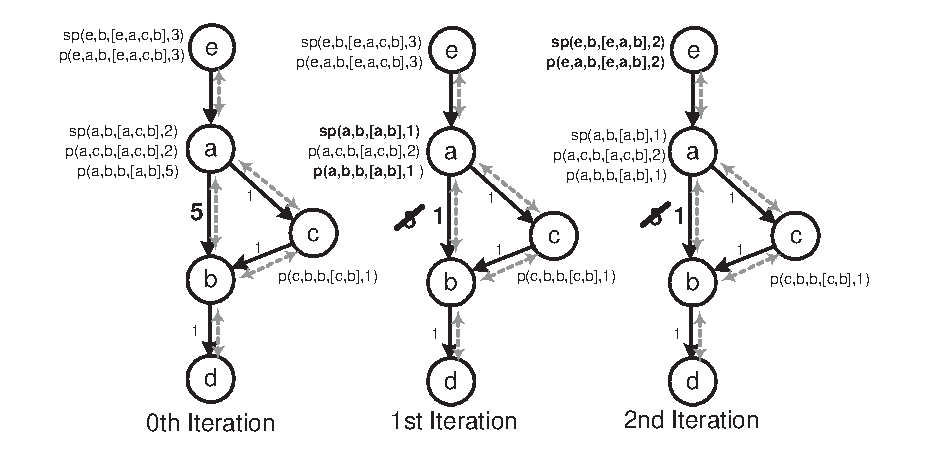
\epsfig{file=images/updateExample.eps, width=3.5in}
%\caption{\label{SP update example}\emph{\small All-Pairs Shortest Path Example
%    with update of link from $link({\bf a},b,5)$ to $link({\bf a},b,1)$. For
%    simplicity, we only show the computed paths and shortest paths to
%    destination node b. The derived tuples that are changed are
%    highlighted in {\em bold}.}}
%\end{figure}                                              

%Having shown incremental maintenance for the centralized case, we step
%through a distributed example, using the same derivation tree as
%before. We use the same network (Figure~\ref{SP update example})
%from our earlier query execution example in
%Section~\ref{sec:queryExec}. In the figure, at the $0^{th}$ iteration
%consists of the computed paths to destination node {\em b}. When
%$link({\bf a},b,5)$ is updated to $link({\bf a},b,1)$,
%$path({\bf a},-,c,[a,c],1)$ is updated at node {\em a}, and
%this results in the computation of $path({\bf e},a,[e,a,b],2)$ which is sent
%to node {\em e}. The shortest paths at each node are also updated
%accordingly to $shortestPath({\bf e},b,[a,b,],1)$ and
%$shortestPath({\bf e},b,[e,a,b],2)$ respectively.

% LocalWords:  recomputations fixpoint Bursty quiesces bursty FP PSN FFP BSN
% LocalWords:  recomputation nextHop stricted
